\chapter{Setup}
In this chapter we explain the setting up of RTDS model and the code for observability analysis and state estimation

%Replace \lipsum with text.
% You may have as many sections as you please. This is just for reference.

\section{RTDS}
RTDS \cite{rtds} is a popular simulation hardware used to run real time power line simulations. It is commonly  used for studies of protective relays, control systems, power hardwares, etc. We use this hardware primarily to simulate a Transmission line and generate and record data for further analysis, such as observability analysis, state estimation, Optimum Power Flow, etc.\\
RSCAD is a simulation software that is used to create models of power lines, to work on the RTDS Simulator Hardware. For our project we set up a model for a 14 bus power line system, with specifications taken from IEEE 14 Bus power system \cite{IEEE14bus}. The model has the following characteristics:
\begin{itemize}
\item Number of Buses: 14
\item Number of Lines: 20
\item Number of Generators: 5
\end {itemize}
The overall system that we designed looked like Figure ~\ref{fig:ckt}.\\
\begin{figure}[h]
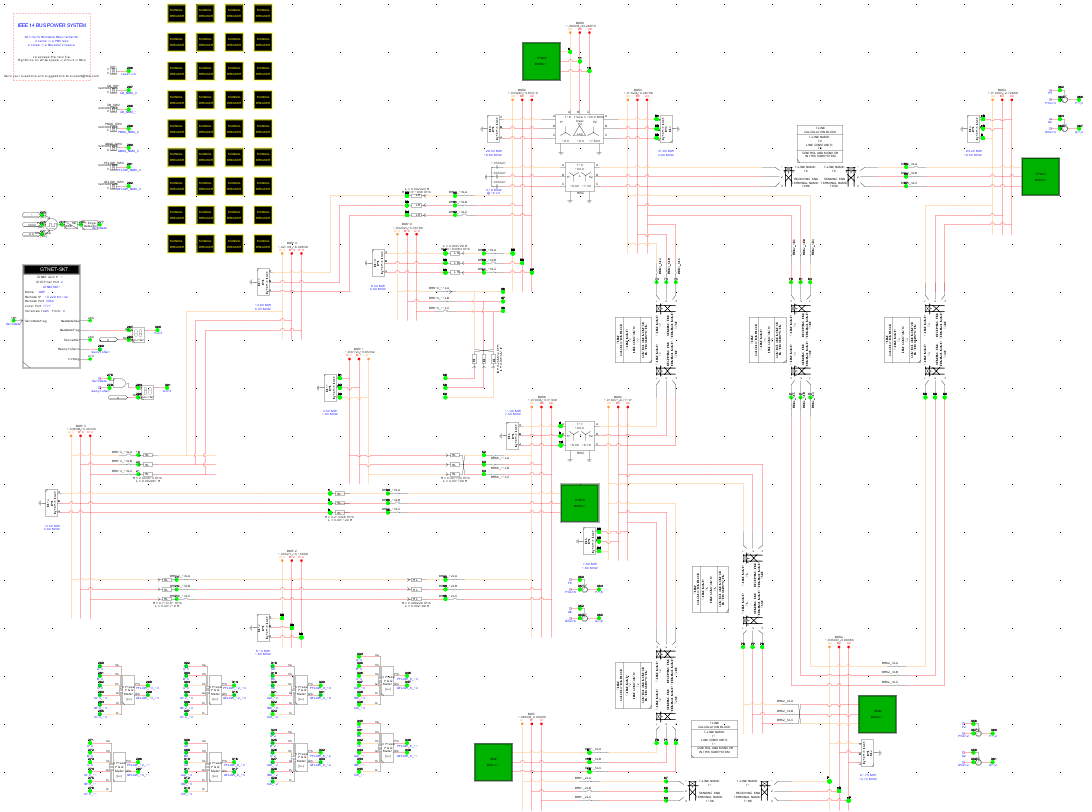
\includegraphics[width=\textwidth]{Figures/ckt.png}
\caption{IEEE 14 Bus Power Line System Model on RSCAD}\label{fig:ckt}
\end{figure}

It had the following key blocks, shown here for reference. (~\ref{fig:bus} to ~\ref{fig:skt})

\begin{figure}[h]
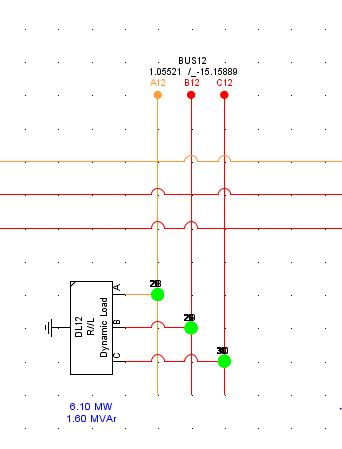
\includegraphics[width=\textwidth]{Figures/bus.jpg}
\caption{Typical Bus in RSCAD}\label{fig:bus}
\end{figure}

\begin{figure}[h]
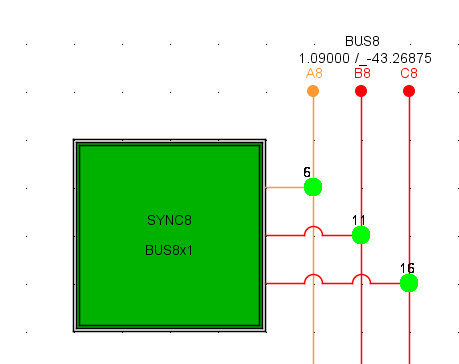
\includegraphics[width=\textwidth]{Figures/gen.png}
\caption{Generator Block in RSCAD}\label{fig:gen}
\end{figure}

\begin{figure}[h]
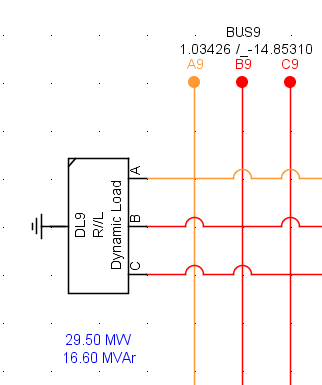
\includegraphics[width=\textwidth]{Figures/load.png}
\caption{PQ load Block in RSCAD}\label{fig:load}
\end{figure}

Apart from the main network, we have the GTNET-SKT block ( Figure ~\ref{fig:skt}), which is crucial for sending and receiving data from RTDS to our server, which records and processes data for further analysis of the power system.  To function, it needs the following parameters specified:
\begin{itemize}
\item All the signals to be measured. In our case, these were the status about all the circuit breakers in the system, the real and complex power injections, real and complex power flows in the lines, and status about availability of each measurement
\item The remote IP address and port of the server to which data is to be sent. 
\end{itemize}
GTNET-SKT 
To simulate real life situations where all data measurements are not available, we also toggle the availability of measurements recorded by GTNET-SKT. Furthermore, we calculate and transmit measurements we call \emph{status numbers}, which provide us information about which measurements are available, and which are not.
\begin{figure}[h]
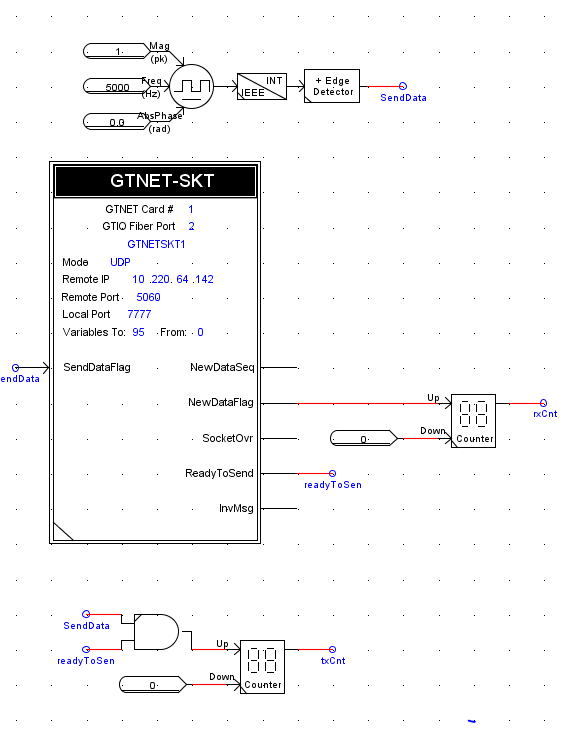
\includegraphics[width=\textwidth]{Figures/skt.png}
\caption{GTNET-SKT Block in RSCAD}\label{fig:skt}
\end{figure}



\section{SECTION NAME}
\lipsum[3]

\section{SECTION NAME}
\lipsum[2]